\documentclass{article}
\usepackage{graphicx,url}
\usepackage[brazil]{babel}
\usepackage[utf8]{inputenc}
\usepackage{enumerate}
\usepackage{tabularx}
\usepackage{multirow}
\usepackage{amsmath}
\usepackage[table,xcdraw]{xcolor}

\title{Protocolo da Revisão Sistemática\\
Ferramentas para Relatório de Negócio com Suporte à XBRL
}
\author{Vagner Clementino \\
       \url{vagnercs@dcc.ufmg.br}}
\date{Setembro de  2015}


\begin{document}

\maketitle

\section{Introdução}
\label{sec:intro}

Uma \textit{Revisão Sistemática da Literatura} - SLR (do inglês Systematic Literature Review) é uma
metodologia científica cujo objetivo é identificar, avaliar e interpretar
\textit{toda} pesquisa \textit{relevante} sobre uma questão de
pesquisa, área ou fenômeno de
interesse\cite{keele2007guidelines,wohlin2012experimentation}. Por se tratar de uma metodologia científica deve estar amparada por um processo conciso para a sua correta execução. Neste sentido, trabalhos que descrevem boas práticas na condução de uma SLR salientam a necessidade da definição de um protocolo durante a fase de planejamento de uma Revisão \cite{keele2007guidelines, biolchini2005systematic}.

Neste contexto, o presente documento tem por objetivo propor um conjunto de diretrizes a serem seguidas durante a condução de uma Revisão Sistemática da literatura sobre o tema \textit{ferramentas para Relatórios de Negócio com suporte à linguagem XBRL}. \textit{Relatórios  de Negócio (Business Report)} é o produto final do  processo de divulgação pública de dados operacionais e financeiras de uma organização ou ainda a prestação regular de informações para os gestores dentro de uma empresa visado apoiá-los no processo de tomada de decisão.
\cite{lymer1999business}. Há uma terceira via da área de  Relatórios de Negócio está relacionada ao processo de prestação de contas por entes públicos aos governos nacionais. A XBRL (\textit{eXtensible Relatórios de Negócio Language}) é uma linguagem para divulgação e intercâmbio de informações financeiras baseada em XML\cite{xbrl_conceitos_aplicacoes}. O padrão vem sendo adotado por diversas instituições e empresas em todo mundo com o suporte de um consórcio global\footnote{\url{www.xbrl.org}} com mais de 650 membros que incentivam a criação de jurisdições locais. Atualmente o consórcio conta com 24 jurisdições, sendo que em países como  Estados Unidos, Grã-Bretanha e Austrália, a XBRL já é a linguagem oficial para entrega
de relatórios à órgãos de governo. A Figura \ref{fig:world_map} exibe os países que estão promovendo a adoção da XBRL. Estes países estão com a coloração mais escura no mapa-múndi.

\begin{figure}[htb]
\centering
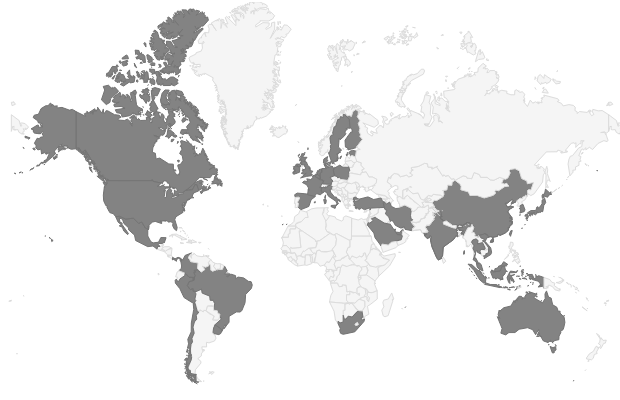
\includegraphics[width=.75\textwidth]{../img/world-map.png}
\caption{O uso da XBRL no mundo}
\label{fig:world_map}
\end{figure}

O protocolo de uma revisão deve especificar o método que será utilizado durante a condução da revisão. Na próximas seções todos os elementos que compõe a Revisão detalhados.


\section{Justificativa}
\label{sec:justificativa}

Tendo em vista determinação da Secretaria do Tesouro Nacional, órgão
vinculado ao  Ministério da Fazenda do Brasil, que definiu o XBRL como
padrão para o envio de relatórios de prestação de contas pelos entes
federativos (estados e municípios) por meio do SICONFI – Sistema de Informações Contábeis e Fiscais do Setor Público Brasileiro \cite{nt_03_2013}, surge a necessidade por parte
daquelas organizações do \textit{desenvolvimento ou aquisição} de sistemas de
informação capazes de criar, processar e enviar informações no formato
XBRL. Um cenário onde tal situação ocorre tal necessidade é latente é em prefeituras de cidades de pequeno e médio porte que necessitam prestar contas via \textit{XBRL}, contudo
não possuem conhecimento ou tempo necessário para desenvolver alguma ferramenta que suporte a linguagem.

Neste sentido, verifica-se que existe a demanda por parte das organizações, especialmente as entidades públicas, de referências de qualidade sobre o assunto de \textit{XBRL}. Neste contexto, entende-se que uma Revisão Sistemática da Literatura - SLR  que avaliasse as ferramentas para Business Report que dão suporte ao XBRL pode \textit{subsidiar a tomada de decisão} por parte dos gestores públicos sobre a aquisição de tais ferramentas. Além disso, um trabalho neste sentido poderia subsidiar o desenvolvimento de novas ferramentas que venham preencher as eventuais lacunas existentes nos sistemas atuais. Ademais, traz o foco da comunidade científica sobre um assunto que vêm crescendo bastante nos últimos anos, dentre outros motivos, devido à necessidade das organizações públicas ou privadas de serem cada vez mais transparentes.


\section{Questões de Pesquisa}
\label{sec:questoes_pesquisa}

A mola-mestra de uma Revisão Sistemática da Literatura é o conjunto de questões de pesquisa ao qual ela se propõe responder. Todo o processo de execução da Revisão tem como base, em último caso, as questões de pesquisa. Para esta revisão são propostas as seguintes questões:

\begin{itemize}
  \item \textbf{$Q1$}: Quais são as ferramentas para Relatórios de Negócio que
    suportam a XBRL?
  \item \textbf{$Q2$}: Quais são os atributos comuns as ferramentas
    que possibilitem a comparação entre elas?
  \item \textbf{$Q3$}: Existem casos reais de utilização da ferramenta
    (Estudos de Casos, Whitepapers e etc)?
  \item \textbf{$Q4$}: Qual setor da economia (governos, medicina, setor financeiro) a ferramenta possui histórico de utilização?
\end{itemize}
A partir deste conjunto de questões é possível propor as sentenças de busca que serão utilizadas na busca dos estudos primários e subsidiar o processo de extração dos dados daqueles estudos.

\section{Estratégia de Busca dos Estudos Primários}
\label{sec:busca_estudos}

Os guias de boas práticas na condução de uma Revisão Sistemática, especialmente
os da medicina, pregão a necessidade de uma busca exaustiva em diversos tipos
de bases de dados, sejam elas eletrônicas ou não. Não obstante, devido à
evolução das ferramentas de indexação de trabalhos acadêmicos, uma revisão pode
utilizar apenas base de dados eletrônicas sem perda de generalidade. Neste
trabalho, serão utilizadas as bases de dados constantes da Tabela
\ref{tab:base-dados} . Trata-se de uma lista com pequenas alteração daquela
proposta por \cite{Brereton2007571} com a inclusão de algumas bases,
especialmente o \textit{Google Scholar} e  \textit{XBRL Consortium}, sendo este
último devido ser o site da entidade mantenedora do XBRL.

\begin{center}
\begin{tabular}{cll}
\label{tab:base-dados}
 Nº&Base de Dados&URL\\
\hline
01 & IEEE Xplore  & \url{http://ieeexplore.ieee.org}\\
02 & ScienceDirect  & \url{http://www.sciencedirect.com/}\\
03 & Springer Link & \url{http://link.springer.com/}\\
04 & ACM Digital Library & \url{http://dl.acm.org/}\\
05 & Web of Science & \url{https://www.webofknowledge.com/}\\
06 & CiteSeer & \url{http://citeseerx.ist.psu.edu}\\
07 & Wiley Online Library & \url{http://onlinelibrary.wiley.com/}\\
08 & Scopus Elsevier & \url{http://www.scopus.com/}\\
09 & EL Compendex & \url{http://www.engineeringvillage2.org}\\
10 & Google scholar & \url{https://scholar.google.com}\\
11 &INSPEC  & \url{http://www.iee.org/publish/inspec/}\\
12 &XBRL Consortium & \url{https://www.xbrl.org/}\\
\end{tabular}
\end{center}


Definida as bases de dados que serão consultados é necessário propor as sentenças de buscas que serão aplicadas visando recuperar os estudos primários. Para tanto, foi conduzido um estudo preliminar visando definir um conjunto de termos que possam ser utilizados no processo de busca. Com o tema da revisão é ferramentas de Relatórios de Negócio com suporte à XBRL, naturalmente sentenças como ``XBRL", ``tools", ``Business Report"\footnote{No estudo preliminar foi utilizado apenas termos em língua inglesa} são possíveis candidatos.

A fim de avaliar qual sentença de busca possibilitaria um conjunto de estudos
preliminares com maior relevância para o trabalho, foi realizada um estudo
prévio utilizando a ferramenta de pesquisa Google
Schoolar\footnote{\url{https://scholar.google.com.br/}}. O estudo é bastante
simples, consistindo apenas em registrar o total de artigos recuperados quando
se realiza uma pesquisa com uma sentença $S_n$ qualquer. Utilizou-se a pesquisa
avançada impondo-se a restrição ``com a frase exata''. Cabe ressaltar que não foi utilizado qualquer tipo de filtro na busca (como por exemplo "por data") e os resultados foram classificados por relevância. Apesar do simplicidade deste procedimento, ele possibilita um bom ponto de partida para definirmos a sentenças de busca que futuramente irão possibilitar a recuperação dos estudos preliminares.

A Tabela \ref{tab:sentencas} exibe as sentenças utilizadas bem como o total de artigos recuperados.
\begin{table}[htb]
\centering
\resizebox{\textwidth}{!}{%
\begin{tabular}{clc}
\rowcolor[HTML]{EFEFEF}
{\bf Código da Sentença} & \multicolumn{1}{c}{\cellcolor[HTML]{EFEFEF}{\bf Sentença}} & {\bf Total de Artigos}     \\ \hline
\multicolumn{1}{|c|}{$S_1$} & \multicolumn{1}{l|}{“XBRL”}                                & \multicolumn{1}{c|}{15100} \\ \hline
\multicolumn{1}{|c|}{$S_2$} & \multicolumn{1}{l|}{“XBRL tools”}                          & \multicolumn{1}{c|}{108}  \\ \hline
\multicolumn{1}{|c|}{$S_3$} & \multicolumn{1}{l|}{“XBRL Business Report tools”}          & \multicolumn{1}{c|}{205}  \\ \hline
\multicolumn{1}{|c|}{$S_4$} & \multicolumn{1}{l|}{“XBRL tools marketing”}                & \multicolumn{1}{c|}{0}  \\ \hline
\multicolumn{1}{|c|}{$S_5$} & \multicolumn{1}{l|}{“XBRL Business Report software tools”} & \multicolumn{1}{c|}{0}  \\ \hline
\end{tabular}
}
\caption{Total de artigos por sentença}
\label{tab:sentencas}
\end{table}

Como pode ser observado a sentença $S_1$ é a consulta mais genérica
que poderia ser feita sobre no contexto da XBRL, contudo, é retornado
um total de $15100$ artigos, um valor relativamente pequeno comparado ao total retornado ao realizar consultas com o termo ``XML' por exemplo\footnote{A consulta por XML retorna aproximadamente $3 \times 10^{6}$ artigos}.

Não obstante a sentença $S_3$ se mostrou satisfatória tanto pelo total
de artigos recuperados bem como pela relevância dos mesmo, auferida
pela inspeção manual de alguns resultados. Visando avaliar o impacto
de restringir o ano de publicação na sentença $S_3$ foi realizada um
novo conjunto de buscas no qual foi utilizado o critério de seleção
``artigos a partir do ano $X$'', onde $X$ é um ano a partir de 2003\footnote{A
  pesquisa inicia-se a partir de 2003 tendo em vista que naquele ano foi
  lançada oficialmente a primeira especificação da XBRL (vide \url{http://specifications.xbrl.org/release-history-base-spec-xbrl-2.1.html})}  Os resultados são exibidos na Figura \ref{fig:graph_artigos_ano}{}.

\begin{figure}[h]
\centering
\label{fig:graph_artigos_ano}
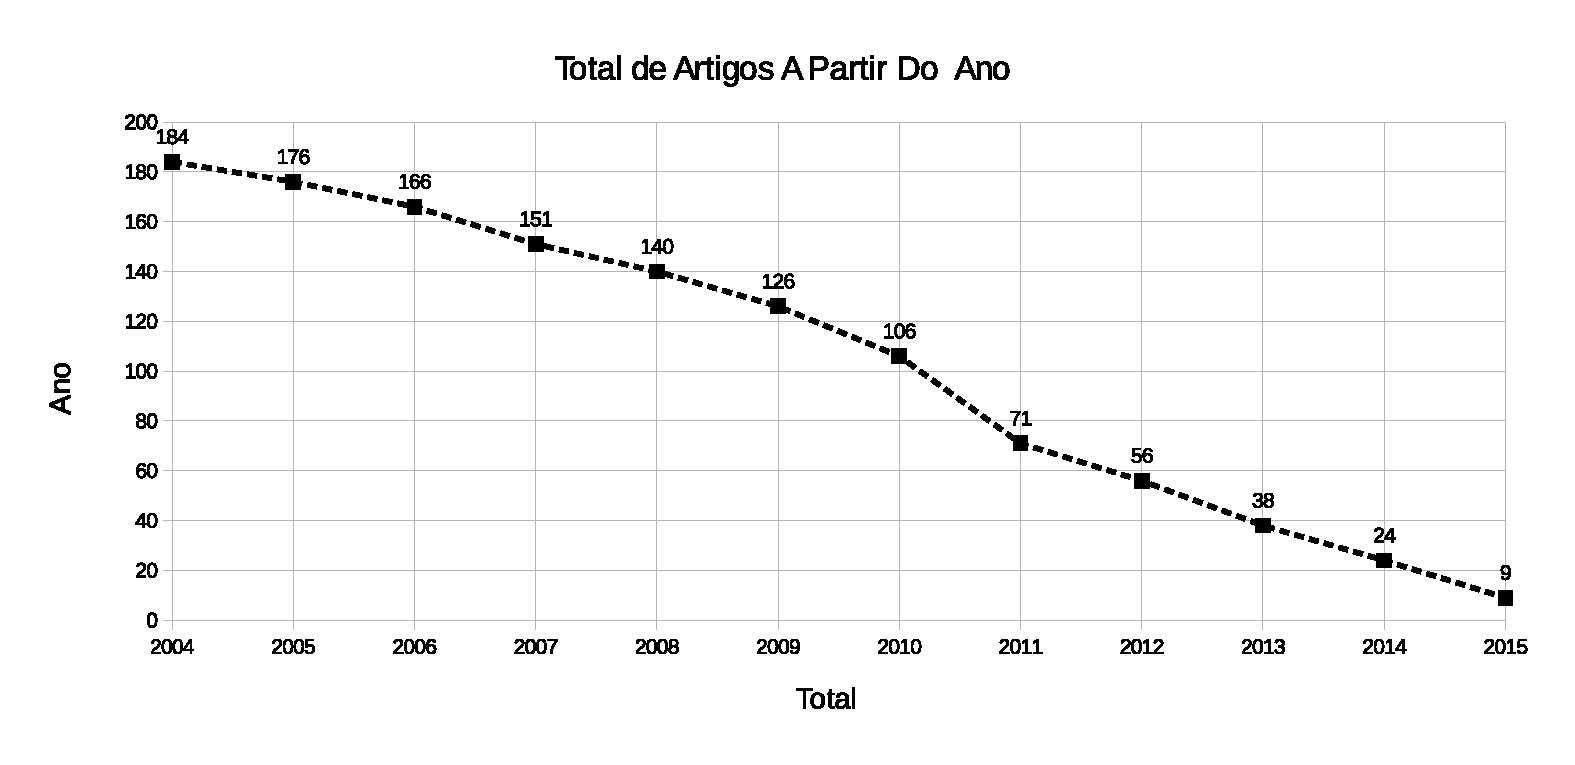
\includegraphics[width=15cm]{../img/graph_01.eps}
\caption{Total de artigo a partir de determinado ano para a sentença $S_3$}
\end{figure}

A Figura \ref{fig:graph_artigos_ano} mostra conforme esperado a
redução do número de artigos quanto se limita o período de
pesquisa. Em uma análise preliminar pode-se afirmar que a utilização
de artigos publicados a partir de \textit{2009} consegue englobar uma massa de
dados suficiente para iniciar a revisão. Além disso em 2009 foi lançada a
versão mais recente da especificação da XBRL\cite{xbrl_conceitos_aplicacoes},
denominada XBRL $2.1$.

Outra ferramenta ser utilizada no processo de coleta dos estudos primários é o
\textit{Dicionários de Sinônimos} que consiste basicamente de um conjunto de
termos similares aos originais que podem aumentar o leque de artigos
recuperados durante a busca. A Tabela \ref{tab:dicionario} exibe o dicionário de dados que deverá ser utilizado durante a Revisão.

\begin{table}[ht]
\centering
\resizebox{\textwidth}{!}{%
\begin{tabular}{|c|l|}
\hline
\multicolumn{2}{|c|}{\textbf{DICIONÁRIO DE SINÔNIMOS}} \\ \hline
\textbf{Termo Original} & \multicolumn{1}{c|}{\textbf{Sinônimo}} \\ \hline
XBRL & XML OR XHTML \\ \hline
software tool & application OR product OR project OR development \\ \hline
Business Report & Finantial Report OR Data Extraction \\ \hline
\end{tabular}
}
\caption{Dicionário de Sinônimos}
\label{tab:dicionario}
\end{table}


\section{Critérios de Inclusão e Exclusão de Estudos}
\label{sec:criterios_in_out}

Nesta seção define-se os critérios para a inclusão de determinado estudo
primário na Revisão. Naturalmente para o estudo ser incluído deverá atender as diretrizes propostas bem
como passar pelo crivo da avaliação de qualidade, conforme disposto na Seção
\ref{sec:qualidade}.

Tendo em vista que os estudo primários serão selecionados de diversas bases de
dados (vide Tabela \ref{tab:base-dados}) possivelmente ocorrerá duplicação de
resultados. Neste sentido o primeiro critério para aceitação de um determinado
estudo é que ele seja único. Para ajudar nesta tarefa poderá ser utilizado
ferramentas para a gestão de referências como por exemplo
\textit{JabRef}\footnote{\url{http://jabref.sourceforge.net/}}.

Finalizada a remoção das possíveis duplicatas o próximo passar é escolher os
artigos que possuem relevância com o tema da revisão utilizando o respectivo
título. Embora o título nem sempre são claros suficientes para  descrever o conteúdo de um trabalho, este processo ajuda a reduzir o conjunto inicial de
estudos primários. Não obstante, caso exista qualquer dúvida quando a
inclusão/exclusão de determinado trabalho este deverá ser marcado para revisão
por outro especialista.

Os artigos que forem incluídos segundo o critério do parágrafo anterior deverão
ser reavaliados com base em seu resumo (\textit{abstract}). Da mesma forma,
deve ser verificado se o resumo do trabalho está condizente com o tema da
Revisão Sistemática. Eventuais dúvidas poderão ser sanadas mediante a revisão
em pares.

Os trabalhos que tiveram aprovação nas três etapas anteriores deverá ter sua
qualidade avaliada conforme proposto na Seção \ref{sec:qualidade}.

\section{Avaliação da Qualidade}
\label{sec:qualidade}

Preferencialmente serão utilizados artigos publicados em conferências ou
journals. Todavia, deverão ser considerados referências relativas à capítulo de
livro. Como partimos da premissa que assunto XBRL é ainda pouco explorado,
entende-se que estudos definidos como literatura cinza (gray literature) -
relatórios técnicos, teses, anais de conferências -  podem
sem incluídos. Apesar das diretrizes de condução de Revisão Sistemática sugere
que este tipo de estudo seja excluído durante a fase de avaliação de qualidade
\cite{keele2007guidelines}, cerca de $9\%$ das evidências obtidas em SLR's
advém de literatura cinza\cite{yasin2012quality}.

\section{Extração dos Dados}
\label{sec:extracao_dados}


TODO. AGUARDANDO SUGESTÕES.


\section{Estratégia de Disseminação}
\label{sec:dissiminacao}
O resultados da Revisão Sistemática serão consolidados em um artigo a ser
apresentado ao alunos da disciplina Engenharia de Software Experimental do
Programa de Pós Graduação em Ciência da Computação da Universidade Federal de
Minas Gerais(UFMG). Posteriormente o trabalho poderá ser revisto visando a
publicação em conferências ou periódicos.
\section{Cronograma}
\label{sec:cronograma}


A Tabela \ref{tab:cronograma} exibe o cronograma de execução da revisão, considerando
também as etapas de apresentação do relatório produzido pela mesma.

\begin{table}[htb]
\centering
\resizebox{\textwidth}{!}{%
\begin{tabular}{|c|l|c|c|}
\hline
\textbf{\#} & \multicolumn{1}{c|}{\cellcolor[HTML]{9B9B9B}\textbf{Atividade}}                                                                           & \cellcolor[HTML]{9B9B9B}\textbf{Previsão Início} & \cellcolor[HTML]{9B9B9B}\textbf{Previsão Término} \\ \hline
01          & Enviar proposta de trabalho via EasyChair                                                                                                 & \textit{05/10/2015}                              & \textit{05/10/2015}                               \\ \hline
02          & Coletar estudos primários com base no estudo preliminar & \textit{06/10/2015}                              & \textit{09/10/2015}                               \\ \hline
03          & Desenvolver o Protocolo da Revisão                                                                                                        & \textit{04/11/2015}                              & \textit{06/11/2015}                               \\ \hline
04          & Revisar o Protocolo com o orientador                                                                                                      & \textit{06/11/2015}                              & \textit{06/11/2015}                               \\ \hline
05          & Aplicar correções sugeridas pelo orientador                                                                                               & \textit{07/11/2015}                              & \textit{08/11/2015}                               \\ \hline
06          & Revisar o Protocolo com o orientador                                                                                                      & \textit{09/11/2015}                              & \textit{09/11/2015}                               \\ \hline
07          & Coletar estudos primários                                                                                                                 & \textit{10/11/2015}                              & \textit{17/11/2015}                               \\ \hline
08          & Selecionar estudos primários                                                                                                              & \textit{18/11/2015}                              & \textit{25/11/2015}                               \\ \hline
09          & Avaliar a qualidade dos estudos primários                                                                                                 & \textit{26/11/2015}                              & \textit{28/11/2015}                               \\ \hline
10          & Extrair dados do estudos primários                                                                                                        & \textit{29/11/2015}                              & \textit{30/11/2015}                               \\ \hline
11          & Escrever Relatório Final                                                                                                                  & \textit{30/11/2015}                              & \textit{02/12/2015}                               \\ \hline
12          & Revisar Relatório Final                                                                                                                   & \textit{02/12/2015}                              & \textit{03/12/2015}                               \\ \hline
13          & Enviar Relatório Final via EasyChair                                                                                                      & \textit{04/12/2015}                              & \textit{04/12/2015}                               \\ \hline
14          & Revisar os outros trabalhos do Workshop                                                                                                   & \textit{07/12/2015}                              & \textit{11/12/2015}                               \\ \hline
15          & Apresentar o Relatório Final no Workshop                                                                                                  & \textit{14/12/2015}                              & \textit{16/12/2015}                               \\ \hline
\end{tabular}
}
\caption{Atividades de execução da SLR}
\label{tab:cronograma}
\end{table}

\pagebreak

\medskip
\bibliographystyle{unsrt}%Used BibTeX style is unsrt
\bibliography{../bib/protocolo_slr_xbrl}

\end{document}
